\documentclass[12pt,a4paper]{beamer}
\usepackage{setspace}
\usepackage[utf8x,utf8]{inputenc}
\usepackage[ngerman]{babel}
\usepackage{ucs}
\usepackage{amsmath}
\usepackage{amsfonts}
\usepackage{amssymb}
\usepackage{lmodern}
\usepackage{hyperref}
\usepackage{verbatim}

% Beamer Settings
\usetheme{Singapore}
\setcounter{tocdepth}{2}

\setbeamertemplate{blocks}[rounded]
\setbeamercolor{block title}{bg=blue!10} 
\setbeamercolor{block body}{bg=blue!30} 

% Default Presentation Settings
\title{Remote Logging mit rsyslog}
\subtitle{Inklusive Tools zur Überwachung und Verwaltung}
\author{Thomas Merkel \and Arkadiusz Rawa \and Janik Lemcke}
\institute{Hochschule Ravensburg-Weingarten}
\date{\today} 

\AtBeginSection[]{%
	\begin{frame}<beamer>
		\frametitle{Inhalt}
		\tableofcontents[sectionstyle=show/hide,subsectionstyle=hide/show/hide]
	\end{frame}
	\addtocounter{framenumber}{-1}% If you don't want them to affect the slide number
}

\begin{document}
	% Intro
	\begin{frame}
		\titlepage
	\end{frame} 
	\begin{frame}
		\frametitle{Inhaltsverzeichnis}
		\tableofcontents[hideallsubsections]
	\end{frame}
	
	% Presentation Parts
	\section{Remote Logging}
\subsection{Problem}
\begin{frame}[plain]
	\frametitle{Remote Logging}
	\framesubtitle{Problem}
	\begin{center}
		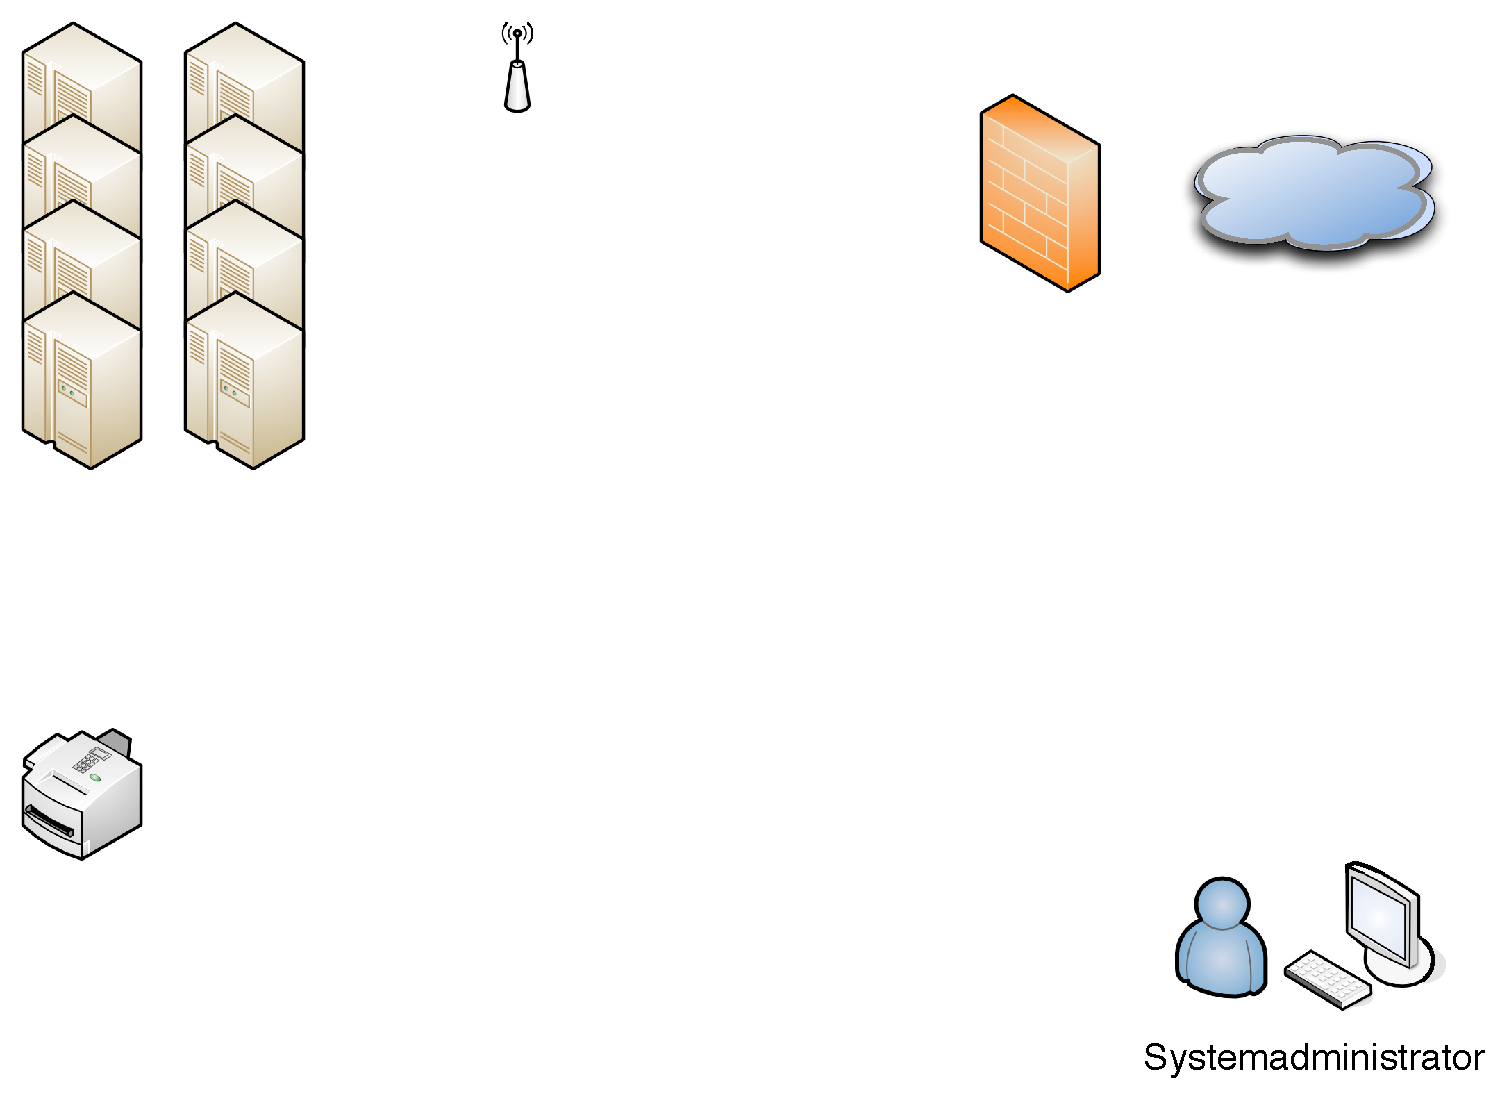
\includegraphics[width=\linewidth]{images/remote_logging_01.eps}
	\end{center}
\end{frame}

\subsection{Panic}
\begin{frame}[plain]
	\frametitle{Remote Logging}
	\framesubtitle{Panic}
	\begin{center}
		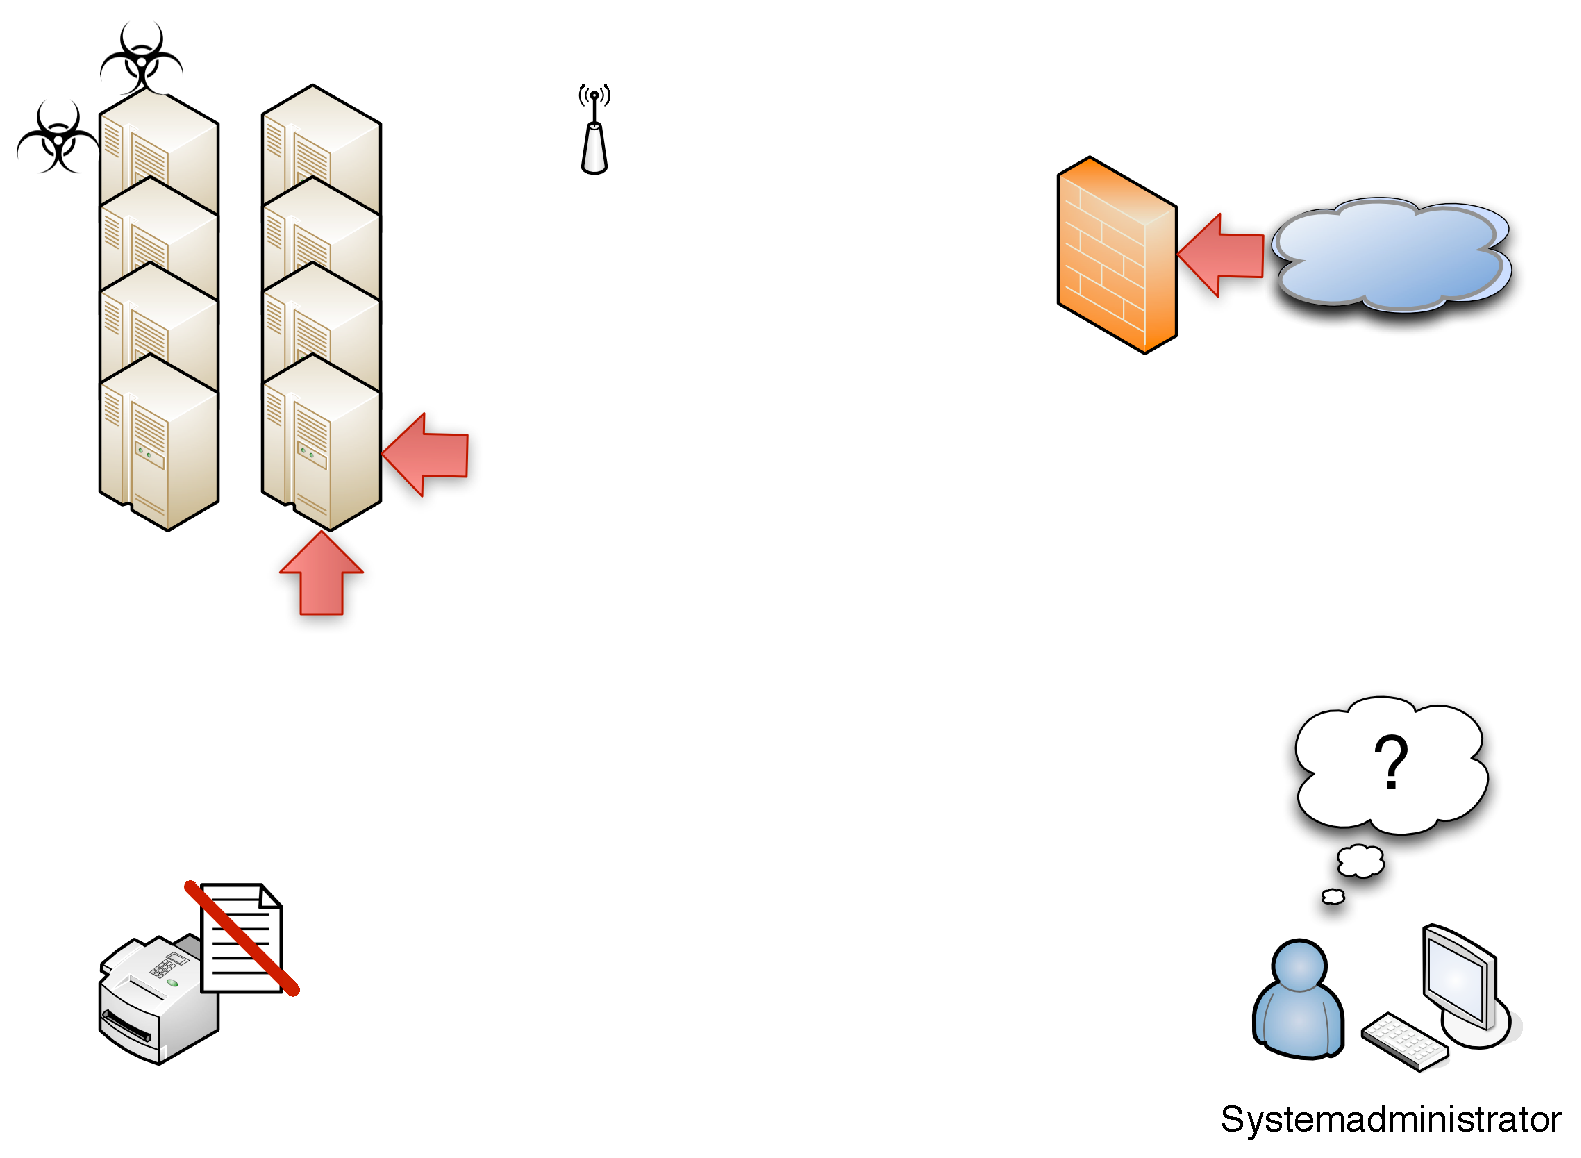
\includegraphics[width=\linewidth]{images/remote_logging_02.eps}
	\end{center}
\end{frame}

\subsection{Don't Panic}
\begin{frame}[plain]
	\frametitle{Remote Logging}
	\framesubtitle{Don't Panic}
	\begin{center}
		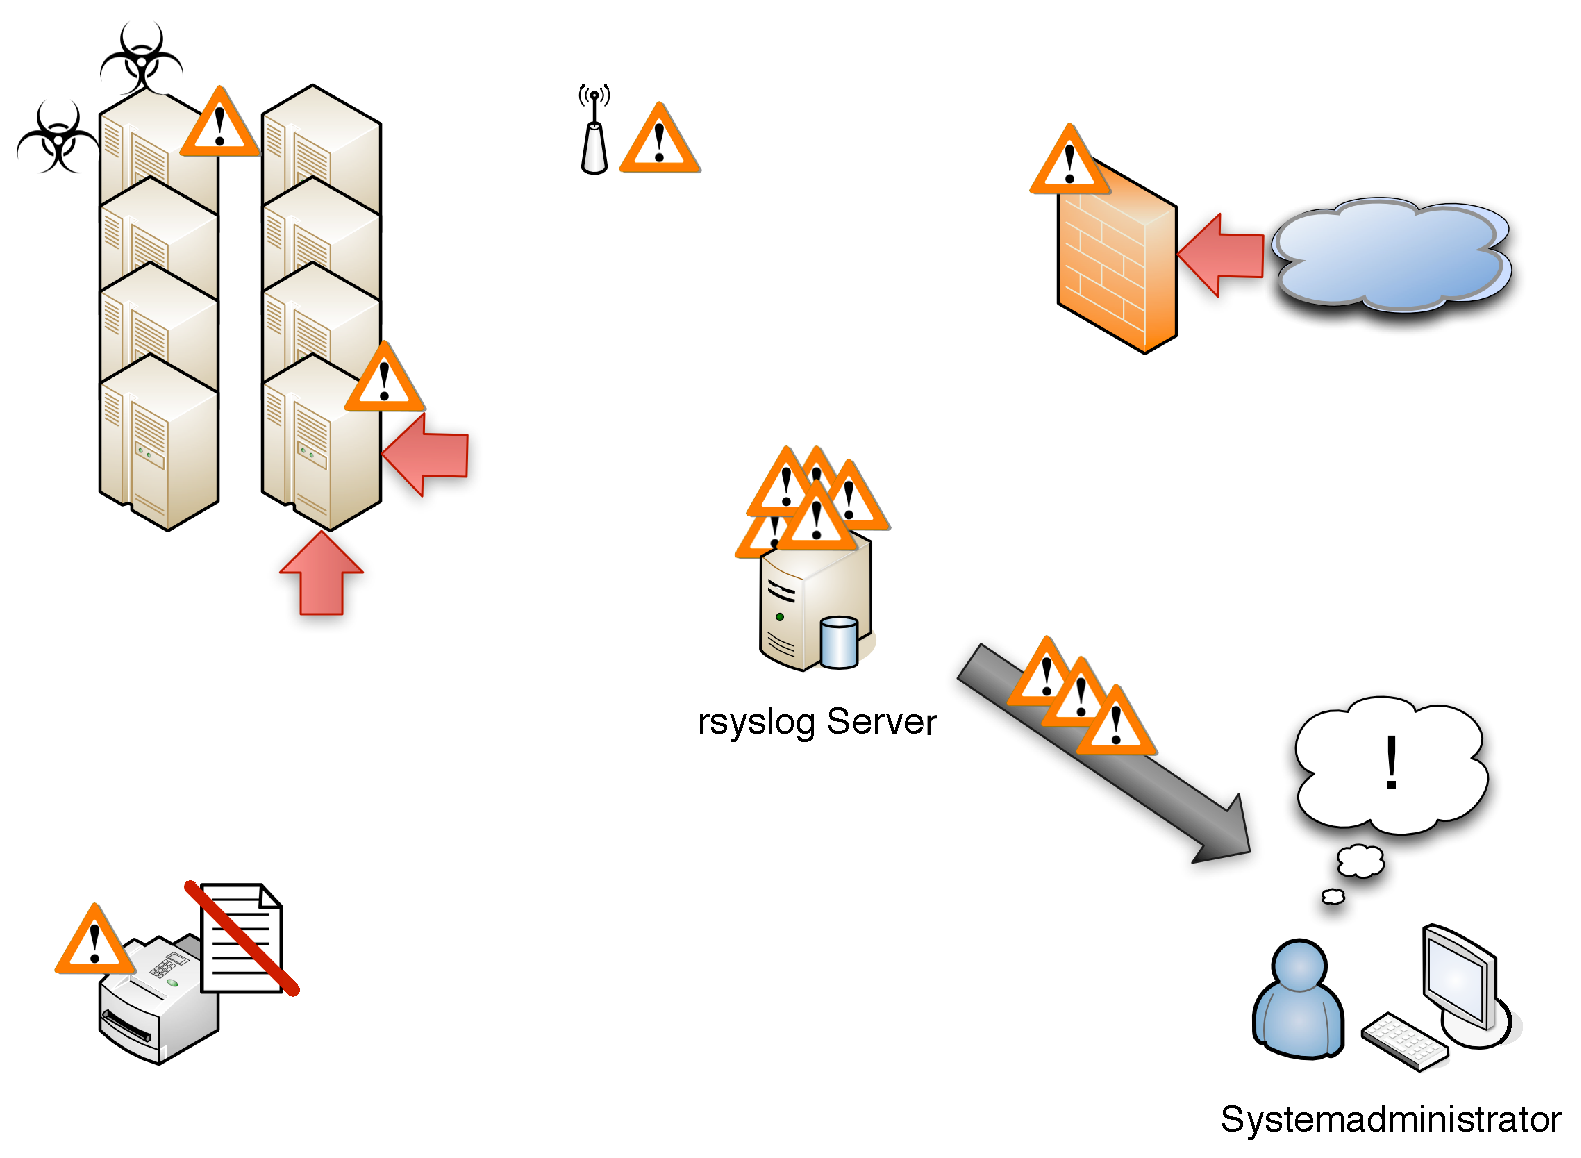
\includegraphics[width=\linewidth]{images/remote_logging_03.eps}
	\end{center}
\end{frame}

\subsection{Ziele}
\begin{frame}
	\frametitle{Remote Logging}
	\framesubtitle{Ziele}
	\begin{itemize}
		\item Alle Informationen an einem zentralen System
		\item Archivierung ist zentralisiert
		\item Alarmierung
		\item Monitoring
	\end{itemize}
\end{frame}
	\section{rsyslog}
\subsection{Überblick}
\begin{frame}[fragile]
	\frametitle{rsyslog}
	\framesubtitle{"Uberblick}
	\begin{itemize}
		\item Alternativer syslog-Daemon
		\item Standard bei Debian-basierten Distributionen
	\end{itemize}
	\begin{center}
		\begin{block}{}
			\begin{tiny}
				\begin{verbatim}
	2011-06-13T10:14:50 bayamo rsyslogd: -- MARK --
	2011-06-13T10:14:55 bayamo sshd[11015]: Accepted publickey for tm from 172.22.175.51 port 49425
	2011-06-13T10:14:55 bayamo sshd[11015]: pam_unix(sshd:session): session opened for user tm uid=0
	2011-06-13T10:14:56 bayamo sudo:       tm : TTY=pts/0 ; PWD=/home/tm ; USER=root ; COMMAND=/bin/su
	2011-06-13T10:14:56 bayamo su[11083]: Successful su for root by root
	2011-06-13T10:14:56 bayamo su[11083]: + /dev/pts/0 root:root
	2011-06-13T10:14:56 bayamo su[11083]: pam_unix(su:session): session opened for user root by tm
				\end{verbatim}
			\end{tiny}
		\end{block}
	\end{center}
\end{frame}

\subsection{Vorteile}
\begin{frame}
	\frametitle{rsyslog}
	\framesubtitle{Vorteile}
	\begin{itemize}
		\item Bessere Sicherheitskontrolle
		\item Mehr Möglichkeiten für die Filterung
		\item Einfaches remote logging
		\item Protokollieren in die Datenbank
	\end{itemize}
\end{frame}

\subsection{Installation}
\begin{frame}[fragile]
	\frametitle{rsyslog}
	\framesubtitle{Installation}
	Paketmanager des Systems ist zu empfehlen
	\bigskip
	\begin{block}{Debian, Ubuntu}
		\begin{verbatim}
			apt-get install rsyslog
		\end{verbatim}
	\end{block}
\end{frame}

\subsection{Konfiguration}
\subsubsection{Konfigurationsdateien}
\begin{frame}[fragile]
	\frametitle{rsyslog}
	\framesubtitle{Konfigurationsdateien}
	\begin{block}{Dateien und Verzeichnisse}
		\begin{verbatim}
			/etc/rsyslog.conf
			/etc/rsyslog.d/*.conf
		\end{verbatim}
	\end{block}
	Sortierung erfolgt durch Nummerierung:
	\begin{itemize}
		\item \verb|/etc/rsyslog.d/00-AllowedHosts.conf|
		\item \verb|/etc/rsyslog.d/10-RemoteLinuxServers.conf|
		\item \verb|/etc/rsyslog.d/99-Default.conf|
	\end{itemize}
\end{frame}

\subsubsection{Remote Logging aktivieren}
\begin{frame}[fragile]
	\frametitle{rsyslog (server)}
	\framesubtitle{Remote Logging aktivieren}
	In \verb|/etc/rsyslog.conf|, folgende Zeile einfügen:
	\begin{block}{}
		\begin{verbatim}
			$ModLoad imudp
			$UDPServerRun 514
		\end{verbatim}
	\end{block}
\end{frame}
\begin{frame}[fragile]
	\frametitle{rsyslog (Server)}
	\framesubtitle{Remote Logging aktivieren}
	Zugriffssteuerung in \verb|/etc/rsyslog.d/00-AllowRemoteLogging.conf|
	\begin{block}{}
		\begin{verbatim}
			# Ein Host
			$AllowedSender UDP, 192.168.56.100
			# Alle Hosts aus einem Subnetz
			$AllowedSender UDP, 192.168.56.0/24
			# Jeder von kernel.org
			$AllowedSender UDP, *.kernel.org
		\end{verbatim}
	\end{block}
\end{frame}

\begin{frame}[fragile]
	\frametitle{rsyslog (Linux Client)}
	\framesubtitle{Remote Logging aktivieren}
	Eintrag in \verb|/etc/rsyslog.d/00-RemoteLogging.conf|
	\begin{block}{}
		\begin{verbatim}
			*.*		@192.168.56.1
		\end{verbatim}
	\end{block}
	Viele syslog-Daemons werden unterstützt
\end{frame}

	\part{tenshi}

	\part{phpLogCon}


	% Last Slide
	\section{Diskussion}
	\begin{frame}
		\frametitle{Diskussion}
		\framesubtitle{Fragen, Anregungen, Wünsche}
		\begin{itemize}
			\item Workshop am nächsten Termin der Linux User Group Weingarten
			\item Alle Unterlagen unter \url{https://github.com/drscream/rsyslog-workshop}
		\end{itemize}
		\bigskip
		\bigskip
		\scriptsize{
			Danke an Paul Nijjar für seine Präsentation: \linebreak 
			\textit{Remote Logging with Rsyslog - How I Learned to Start Worrying and Love the Panopticon}
		}
	\end{frame}
\end{document}